% Options for packages loaded elsewhere
\PassOptionsToPackage{unicode}{hyperref}
\PassOptionsToPackage{hyphens}{url}
%
\documentclass[
  12pt,
]{article}
\usepackage{amsmath,amssymb}
\usepackage{lmodern}
\usepackage{iftex}
\ifPDFTeX
  \usepackage[T1]{fontenc}
  \usepackage[utf8]{inputenc}
  \usepackage{textcomp} % provide euro and other symbols
\else % if luatex or xetex
  \usepackage{unicode-math}
  \defaultfontfeatures{Scale=MatchLowercase}
  \defaultfontfeatures[\rmfamily]{Ligatures=TeX,Scale=1}
\fi
% Use upquote if available, for straight quotes in verbatim environments
\IfFileExists{upquote.sty}{\usepackage{upquote}}{}
\IfFileExists{microtype.sty}{% use microtype if available
  \usepackage[]{microtype}
  \UseMicrotypeSet[protrusion]{basicmath} % disable protrusion for tt fonts
}{}
\makeatletter
\@ifundefined{KOMAClassName}{% if non-KOMA class
  \IfFileExists{parskip.sty}{%
    \usepackage{parskip}
  }{% else
    \setlength{\parindent}{0pt}
    \setlength{\parskip}{6pt plus 2pt minus 1pt}}
}{% if KOMA class
  \KOMAoptions{parskip=half}}
\makeatother
\usepackage{xcolor}
\usepackage[margin=1in]{geometry}
\usepackage{color}
\usepackage{fancyvrb}
\newcommand{\VerbBar}{|}
\newcommand{\VERB}{\Verb[commandchars=\\\{\}]}
\DefineVerbatimEnvironment{Highlighting}{Verbatim}{commandchars=\\\{\}}
% Add ',fontsize=\small' for more characters per line
\usepackage{framed}
\definecolor{shadecolor}{RGB}{248,248,248}
\newenvironment{Shaded}{\begin{snugshade}}{\end{snugshade}}
\newcommand{\AlertTok}[1]{\textcolor[rgb]{0.94,0.16,0.16}{#1}}
\newcommand{\AnnotationTok}[1]{\textcolor[rgb]{0.56,0.35,0.01}{\textbf{\textit{#1}}}}
\newcommand{\AttributeTok}[1]{\textcolor[rgb]{0.77,0.63,0.00}{#1}}
\newcommand{\BaseNTok}[1]{\textcolor[rgb]{0.00,0.00,0.81}{#1}}
\newcommand{\BuiltInTok}[1]{#1}
\newcommand{\CharTok}[1]{\textcolor[rgb]{0.31,0.60,0.02}{#1}}
\newcommand{\CommentTok}[1]{\textcolor[rgb]{0.56,0.35,0.01}{\textit{#1}}}
\newcommand{\CommentVarTok}[1]{\textcolor[rgb]{0.56,0.35,0.01}{\textbf{\textit{#1}}}}
\newcommand{\ConstantTok}[1]{\textcolor[rgb]{0.00,0.00,0.00}{#1}}
\newcommand{\ControlFlowTok}[1]{\textcolor[rgb]{0.13,0.29,0.53}{\textbf{#1}}}
\newcommand{\DataTypeTok}[1]{\textcolor[rgb]{0.13,0.29,0.53}{#1}}
\newcommand{\DecValTok}[1]{\textcolor[rgb]{0.00,0.00,0.81}{#1}}
\newcommand{\DocumentationTok}[1]{\textcolor[rgb]{0.56,0.35,0.01}{\textbf{\textit{#1}}}}
\newcommand{\ErrorTok}[1]{\textcolor[rgb]{0.64,0.00,0.00}{\textbf{#1}}}
\newcommand{\ExtensionTok}[1]{#1}
\newcommand{\FloatTok}[1]{\textcolor[rgb]{0.00,0.00,0.81}{#1}}
\newcommand{\FunctionTok}[1]{\textcolor[rgb]{0.00,0.00,0.00}{#1}}
\newcommand{\ImportTok}[1]{#1}
\newcommand{\InformationTok}[1]{\textcolor[rgb]{0.56,0.35,0.01}{\textbf{\textit{#1}}}}
\newcommand{\KeywordTok}[1]{\textcolor[rgb]{0.13,0.29,0.53}{\textbf{#1}}}
\newcommand{\NormalTok}[1]{#1}
\newcommand{\OperatorTok}[1]{\textcolor[rgb]{0.81,0.36,0.00}{\textbf{#1}}}
\newcommand{\OtherTok}[1]{\textcolor[rgb]{0.56,0.35,0.01}{#1}}
\newcommand{\PreprocessorTok}[1]{\textcolor[rgb]{0.56,0.35,0.01}{\textit{#1}}}
\newcommand{\RegionMarkerTok}[1]{#1}
\newcommand{\SpecialCharTok}[1]{\textcolor[rgb]{0.00,0.00,0.00}{#1}}
\newcommand{\SpecialStringTok}[1]{\textcolor[rgb]{0.31,0.60,0.02}{#1}}
\newcommand{\StringTok}[1]{\textcolor[rgb]{0.31,0.60,0.02}{#1}}
\newcommand{\VariableTok}[1]{\textcolor[rgb]{0.00,0.00,0.00}{#1}}
\newcommand{\VerbatimStringTok}[1]{\textcolor[rgb]{0.31,0.60,0.02}{#1}}
\newcommand{\WarningTok}[1]{\textcolor[rgb]{0.56,0.35,0.01}{\textbf{\textit{#1}}}}
\usepackage{graphicx}
\makeatletter
\def\maxwidth{\ifdim\Gin@nat@width>\linewidth\linewidth\else\Gin@nat@width\fi}
\def\maxheight{\ifdim\Gin@nat@height>\textheight\textheight\else\Gin@nat@height\fi}
\makeatother
% Scale images if necessary, so that they will not overflow the page
% margins by default, and it is still possible to overwrite the defaults
% using explicit options in \includegraphics[width, height, ...]{}
\setkeys{Gin}{width=\maxwidth,height=\maxheight,keepaspectratio}
% Set default figure placement to htbp
\makeatletter
\def\fps@figure{htbp}
\makeatother
\setlength{\emergencystretch}{3em} % prevent overfull lines
\providecommand{\tightlist}{%
  \setlength{\itemsep}{0pt}\setlength{\parskip}{0pt}}
\setcounter{secnumdepth}{-\maxdimen} % remove section numbering
\usepackage{fancyhdr}
\usepackage{fontspec}
\usepackage{xcolor}
\usepackage{hyperref}
\usepackage{pdfcomment}
\usepackage{datetime}
\usepackage[document]{ragged2e}

\setmainfont{Poppins}

\newdateformat{monthyeardate}{\monthname[\THEMONTH] \THEYEAR}

% header and footer
\fancypagestyle{firstpage}{
\setlength{\headheight}{75pt}
\setlength{\textheight}{600pt}
\fancyhead[C]{}
\fancyhead[L]{
\includegraphics{X:/DSA/Trends/household-travel-survey/headers/PST_2021_HTS_header.png}}
\fancyhead[R]{}

\fancyfoot[L]{\scriptsize{1011 Western Ave, Suite 500, Seattle WA 98104} \textcolor[HTML]{F05A28}. 206.464.7532 \textcolor[HTML]{F05A28}. www.psrc.org \textcolor[HTML]{F05A28}. \monthyeardate\today}
\fancyfoot[R]{\textcolor[HTML]{F05A28}\thepage}
\fancyfoot[C]{}
\renewcommand{\headrulewidth}{0pt}
\renewcommand{\footrulewidth}{4pt}
\renewcommand{\footrule}{\hbox to \headwidth{\color[HTML]{BCBEC0}\leaders\hrule height \footrulewidth\hfill}}
}

\fancypagestyle{otherpages}{
\fancyhead{}
\fancyfoot[L]{\scriptsize{1011 Western Ave, Suite 500, Seattle WA 98104} \textcolor[HTML]{F05A28}. 206.464.7532 \textcolor[HTML]{F05A28}. www.psrc.org \textcolor[HTML]{F05A28}. \monthyeardate\today}
\fancyfoot[R]{\textcolor[HTML]{F05A28}\thepage}
\fancyfoot[C]{}
\renewcommand{\headrulewidth}{0pt}
\renewcommand{\footrulewidth}{4pt}
\renewcommand{\footrule}{\hbox to \headwidth{\color[HTML]{BCBEC0}\leaders\hrule height \footrulewidth\hfill}}
}


\usepackage{xcolor}
\usepackage{hyperref}
\usepackage{pdfcomment}
\usepackage{fancyhdr} \pagestyle{fancy} \setlength{\headheight}{75pt} \setlength{\textheight}{600pt} \fancyhead[C]{} \fancyhead[L]{
\includegraphics{X:/DSA/shiny-uploads/images/PST_Equity_Edition-Trend_header.png}} \fancyhead[R]{} \fancyfoot[L]{\scriptsize{1011 Western Ave, Suite 500, Seattle WA 98104} \textcolor[HTML]{F05A28}. 206.464.7532 \textcolor[HTML]{F05A28}. www.psrc.org \textcolor[HTML]{F05A28}. January 2023} \fancyfoot[R]{\textcolor[HTML]{F05A28}\thepage} \fancyfoot[C]{} \renewcommand{\headrulewidth}{0pt} \renewcommand{\footrulewidth}{4pt} \renewcommand{\footrule}{\hbox to \headwidth{\color[HTML]{BCBEC0}\leaders\hrule height \footrulewidth\hfill}}
\usepackage{fontspec}
\ifLuaTeX
  \usepackage{selnolig}  % disable illegal ligatures
\fi
\IfFileExists{bookmark.sty}{\usepackage{bookmark}}{\usepackage{hyperref}}
\IfFileExists{xurl.sty}{\usepackage{xurl}}{} % add URL line breaks if available
\urlstyle{same} % disable monospaced font for URLs
\hypersetup{
  hidelinks,
  pdfcreator={LaTeX via pandoc}}

\author{}
\date{\vspace{-2.5em}}

\begin{document}

\setmainfont{Poppins}

\hypertarget{womens-travel-needs-often-overlooked}{%
\section{Women's Travel Needs Often
Overlooked}\label{womens-travel-needs-often-overlooked}}

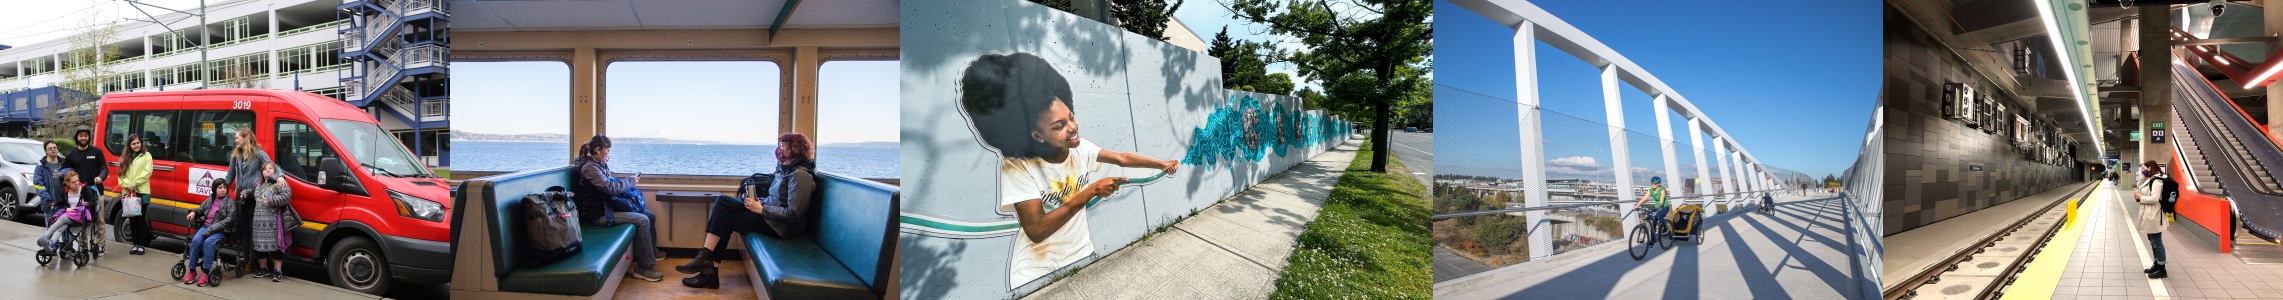
\includegraphics[width=1\textwidth,height=\textheight]{C:/Coding/CURRENT_REPOS_GITHUB/document-maker/templates/equity_example/women2_image_header.png}

\begin{flushleft}
The way in which we design our urban environments oftentimes overlook the needs of families and female-identifying residents. Leslie Kern's book \href{https://metropolismag.com/viewpoints/leslie-kern-feminist-city/}{\underline{\textcolor{blue}{Feminist City}}} explore some of the ways in which we can redesign and shape our cities through a "gender lens." \medskip


Speaking to some of these disparities, in particular, women have \href{http://libraryarchives.metro.net/DB_Attachments/2019-0294/UnderstandingHowWomenTravel_FullReport_FINAL.pdf}{\underline{\textcolor{blue}{transportation needs that have not historically been met}}}. The regional transportation system, including transit, was traditionally designed around the need to quickly get to work at central locations. Women tend to carry significantly more of the care-giving burden's of society and thus need a system that works safely for traveling with others to a variety of locations at all times of day. Women also represent a large portion of older populations who have unique transportation needs that are not well-served by our system built around driving and work destinations. Women are also more likely to live in poverty and have lower incomes than men, which impact many aspects of transit needs and housing needs or limitations.\medskip


As the world trends, in a COVID world, towards greater telecommuting for some people and continued trends in aging, will the transportation system evolve for women?
\end{flushleft}

\hypertarget{puget-sound-regional-household-travel-survey}{%
\paragraph{Puget Sound Regional Household Travel
Survey}\label{puget-sound-regional-household-travel-survey}}

\begin{flushleft}
The 2017, 2019, and 2021 household travel surveys collected day-to-day information from households in the central Puget Sound region, such as how we traveled, where we went, how long it took—even where we chose to live and whether we got home deliveries, prior to COVID-19 and after. \smallskip


This report starts with comparison of travel by gender, during the stable period prior to COVID-19, and then dives into some recent trends that occured in 2021, during COVId-19.  Learn more at the \href{https://www.psrc.org/our-work/household-travel-survey-program}{\underline{\textcolor{blue}{household travel survey webpage}}}. Data from 2017 and 2019 have combined to give a more robust sample size.  You can also \href{https://household-travel-survey-psregcncl.hub.arcgis.com}{\underline{\textcolor{blue}{view the full survey dataset here}}}, including 2017, 2019 and 2021 data. 
\end{flushleft}

\hypertarget{travel-behavior-and-transit-trends}{%
\subsection{Travel Behavior and Transit
Trends}\label{travel-behavior-and-transit-trends}}

\begin{flushleft}
Through the analysis in this report, key trends have emerged that differentiate female-identifying resident’s travel patterns from men’s travel patterns, across all modes. Across all modes, more women are making many more trips (7 or more) per day than men. Inversely, more women than men are also not making any trips per day. This means women may experience more exposure to travel burdens (cost, stress, or safety risks), or may be more likely to be isolated or disconnected from the opportunities that travel affords.

Women’s trips are more varied to a broader spread of destinations, and are more likely to primarily serve the needs of someone else. Women are more likely to live in a car-free or carlight household, take more trips with other people, take fewer single-occupant car trips than men, and are more likely to carpool or get a ride from a family member or friend if they don’t have a driver’s license.

Among female riders, almost 90\% ride the system more than three days per week. Fifty-seven percent of women bring their children on transit, and they often ride transit because they do not have a car, they want to avoid traffic, or because they do not have a license. Two of these three reasons indicate that women who ride transit do so because they have fewer transportation options, and may have less access to economic opportunities as a result. Over 85\% of women riders use Metro to travel to work or school, and of those women, 32\% also use Metro to run errands or complete recreational trips. Among people who make household serving trips most frequently, these trips comprise the same share for women whether they use transit or not; for men, the share of household-serving trips declines if they are transit users. This shows that while men are more likely to find alternatives to using transit to complete household-serving trips (using a different mode or taking fewer trips), women are less likely to find an alternative, and instead work to make the transit system work for their needs. Although the rate of adoption for Transportation Network Companies (TNCs) like Uber and Lyft is the same for men and women, women are more likely than men to report that their transit use has stayed the same as they have also begun to use TNCs. Women are more likely than men to say they use TNCs for trips that transit does not serve, while men are more likely to say they use TNCs to reach a transit stop or station. The trips that are not served by transit may be related to time or location, as women’s needs differ from men’s needs by both time of day and location.
\end{flushleft}

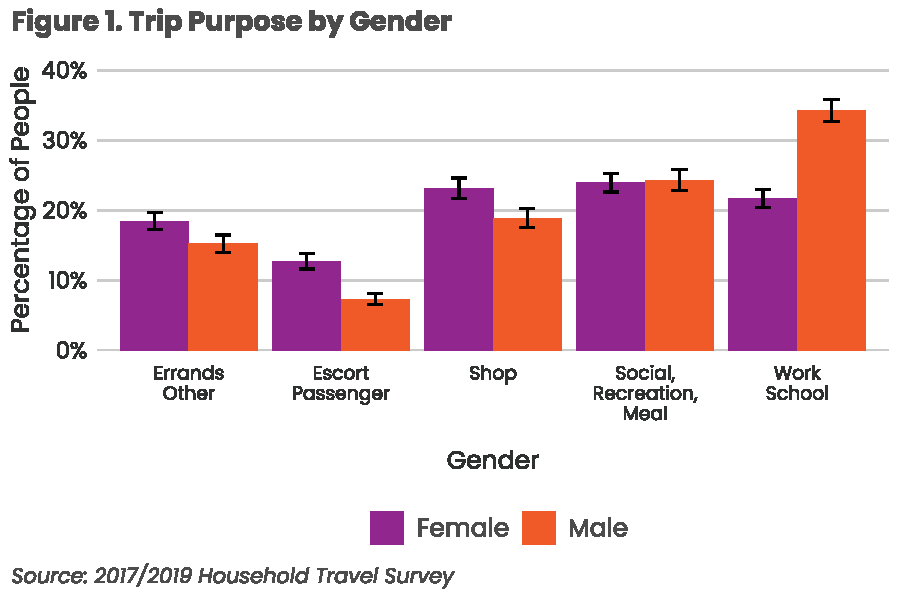
\includegraphics{womens_history_story_draft_files/figure-latex/trip by gender-1.pdf}

\hypertarget{implications-for-womens-limitations-and-access}{%
\paragraph{Implications for Women's Limitations and
Access}\label{implications-for-womens-limitations-and-access}}

\begin{flushleft}
Household Travel Survey Data from 2017 and 2019 combined suggest that women make more trips for care-giving purposes like escorting passengers, shopping, running household errands, and less trips for work and school.


These findings suggest that women are required to adjust their own schedule and travel needs to accommodate others, and in doing so, give up some of their own autonomy and control over when and how they travel. Despite these challenges and tradeoffs, women show ingenuity in arranging their schedules to meet their travel needs. Women are more likely to trip-chain, or make stops along the way to other destinations, and describe consolidating all their errand trips into one day where they will have access to a vehicle.


These travel behavior findings point towards many opportunities to adjust the services provided by Metro to better meet the travel needs expressed by those who are using transit. Development of a Gender Action Plan - or a tactical plan to implement policy, design, and service changes throughout the agency - wouldn help to articulate the immediate opportunities and long-term goals that would create a system that better serves women. Adjustments to services, vehicle design, and policy would help minimize the time, cost, safety, and physical burdens and additional emotional labor of riding transit for the more than half of all riders who are women. Gemma Hartley's book speaks to this added level of acrobatics that women oftentimes face when navigating caretaking, professional, and personal hurdles in \href{https://www.gemmahartley.com/}{\underline{\textcolor{blue}{Fed Up: Emotional Labor, Women and the Way Forward}}}.
\end{flushleft}

\begin{flushleft}
The findings from \href{https://thesource.metro.net/2019/09/19/metro-releases-understanding-how-women-travel-report/}{\underline{\textcolor{blue}{Understanding How Women Travel}}} about women’s mode choices, how likely they are to travel with others in their care, and their complex trip-chaining patterns could all inform adjustments to Metro’s fare policy to make it more equitable towards women and more cost-competitive with driving and carpooling. Findings about women’s trip purposes and primary responsibility for household errands could all inform the way transit vehicles, transit stations, and bus stops are designed, so that space for traveling with others and carrying bags and other belongings could be better accommodated. Findings about when women are traveling and average trip lengths could inform new service offerings that meet a mid-day peak travel demand and provide better direct connections over long distances while minimizing transfers. 

The transportation system, instead, is set up for people to get quickly to work.
\end{flushleft}

\hypertarget{nationwide-data-shows-similar-burdens-and-constraints}{%
\subsection{Nationwide Data Shows Similar Burdens and
Constraints}\label{nationwide-data-shows-similar-burdens-and-constraints}}

\begin{flushleft}
PUMS data shows women are employed more than men, but not to the extent the trip purposes diverge. Women who are working are still carrying more burden of other household tasks.
\end{flushleft}

\begin{flushleft}
Women take shorter more local trips, as opposed to long highway trips. The transportation system needs to be set up for people getting to a variety of locations by a variety of modes.
\end{flushleft}

\begin{Shaded}
\begin{Highlighting}[]
\NormalTok{employ\_\_gender\_chart\_19}
\NormalTok{distance}
\end{Highlighting}
\end{Shaded}

\begin{figure}
\subfloat[Employment\label{fig:matrix-1}]{\includegraphics[width=0.5\linewidth]{womens_history_story_draft_files/figure-latex/matrix-1} }\subfloat[Trip Distance\label{fig:matrix-2}]{\includegraphics[width=0.5\linewidth]{womens_history_story_draft_files/figure-latex/matrix-2} }\caption{Source: ACS 2019 1-year; Sex by Employment Status and 2017/2019 Household Travel SUrvey}\label{fig:matrix}
\end{figure}
\begin{flushleft}
Women in households with more than two people tend to travel more with other people than men. Transit is often not well set up for people who are traveling with strollers. The walk and bike network are not built out for people of all ages to use.
\end{flushleft}

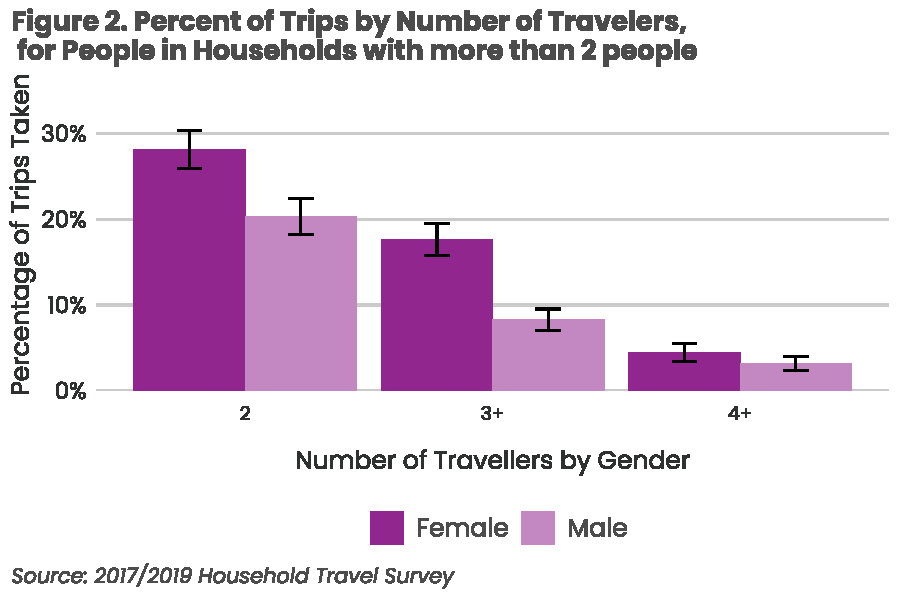
\includegraphics{womens_history_story_draft_files/figure-latex/Trips by Number of Travellers-1.pdf}

\begin{flushleft}
Women represent a greater share of the older population who needs more specialized transportation services, and less service to work locations. \href{https://www.nytimes.com/2022/12/03/health/elderly-living-alone.html}{\underline{\textcolor{blue}{New York Times}}}. Additionally, women, on average, tend to live longer than men, so that at older ages there are many more women who have unique travel needs than men. Older people (who tend to be women more often) have more need for transit in off-peak hours and specialized transportation services. 
\end{flushleft}

\includegraphics{womens_history_story_draft_files/figure-latex/Age group by gender-1.pdf}

\begin{flushleft}
Women bike much less than men. Some of this is undoubtedly because of bike network design does not feel well-suited or safe for all people of different ages and abilities. As a result, in 2019 only 30,000 bike trips were made by women but 74,000 men. How can the transportation and land use system better accommodate older people, household maintenance and caregiving needs? Addressing these questions will improve the system for all genders.
\end{flushleft}

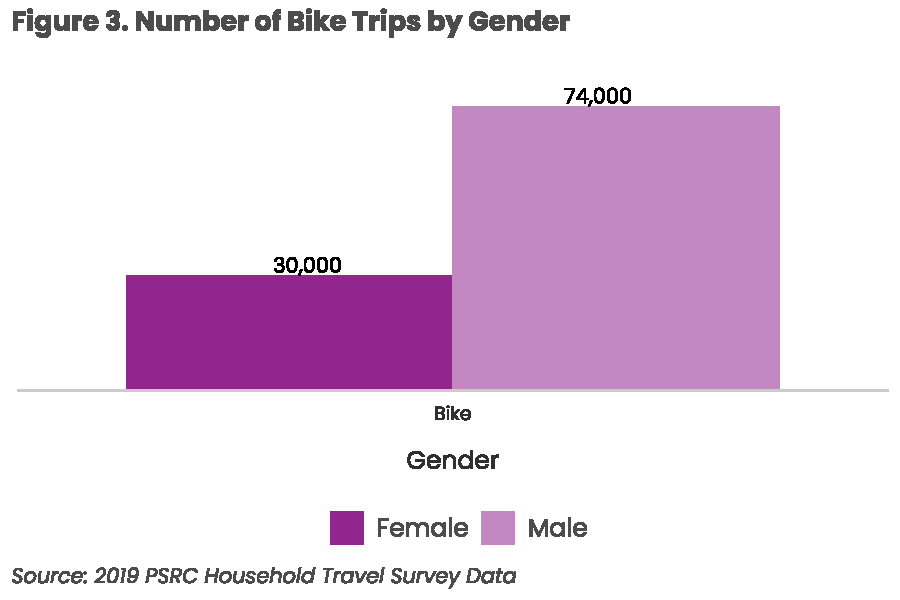
\includegraphics{womens_history_story_draft_files/figure-latex/Bike trips-1.pdf}

\begin{flushleft}
COVID-19 brought about abrupt changes to the transportation landscape. The 2021 Household Travel survey showed big changes in travel behavior. More people were walking and biking, and less people were using transit. Many more people began to telework. Women teleworked more than men, before COVID-19, and the data shows this difference increase even more in 2021. In 2021, 41\% of women teleworked, as compared to 33\% of men. The difference between telework rates relates to women's job sectors as compared to men, and also household responsibilities.
\end{flushleft}

\begin{verbatim}
## Scale for x is already present.
## Adding another scale for x, which will replace the existing scale.
\end{verbatim}

\includegraphics{womens_history_story_draft_files/figure-latex/2017/2019 to 2021-1.pdf}

\begin{flushleft}
In 2021, people were traveling for different purposes.
\end{flushleft}

\includegraphics{womens_history_story_draft_files/figure-latex/2017/2019 to 2021 trips-1.pdf}

\begin{flushleft}
What else?



\subsection{Conclusion}

someotherwords
\end{flushleft}

\end{document}
